\documentclass[10pt]{beamer}

\usetheme{metropolis}
\usepackage{appendixnumberbeamer}

\usepackage{booktabs}
\usepackage[scale=2]{ccicons}

\usepackage{amsmath}
\usepackage{amssymb}

\usepackage{pgfplots}
\usepgfplotslibrary{dateplot}

\usepackage{mathtools} % Mathe
\usepackage{amsfonts} % Mathesymbole

\usepackage{xspace}
\newcommand{\themename}{\textbf{\textsc{metropolis}}\xspace}
\newcommand{\indep}{\rotatebox[origin=c]{90}{$\models$}}

\title{Attacking and Improving Invert and Classify Defense}
\date{May 3, 2018}
\author{Justin Lewis, Jeong-Yeol Kwon, Dany Haddad}
% \institute{}
% \titlegraphic{\hfill\includegraphics[height=1.5cm]{logo.pdf}}


\begin{document}


\maketitle

\begin{frame}{Refresher on Adversarial Examples for Image Classification}
\begin{figure}[H]
    \caption{Adversarial examples for an MNIST classifier}
    \centering
    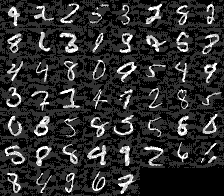
\includegraphics[scale=0.5]{./cl_adversarial.png}
\end{figure}
    \begin{itemize}
        \item Perturb a natural image slightly to fool a classifier
        \item We expect that natural images exist in a low dimensional manifold
        \item These examples are typically far from the manifold of natural images \cite{ilyas2017}
        \item The classifier has not been trained on images outside this manifold
    \end{itemize}
\end{frame}

\begin{frame}[fragile]{Invert and Classify Defense}
    \begin{figure}[H]
    \caption{the INC defense method}
    \centering
    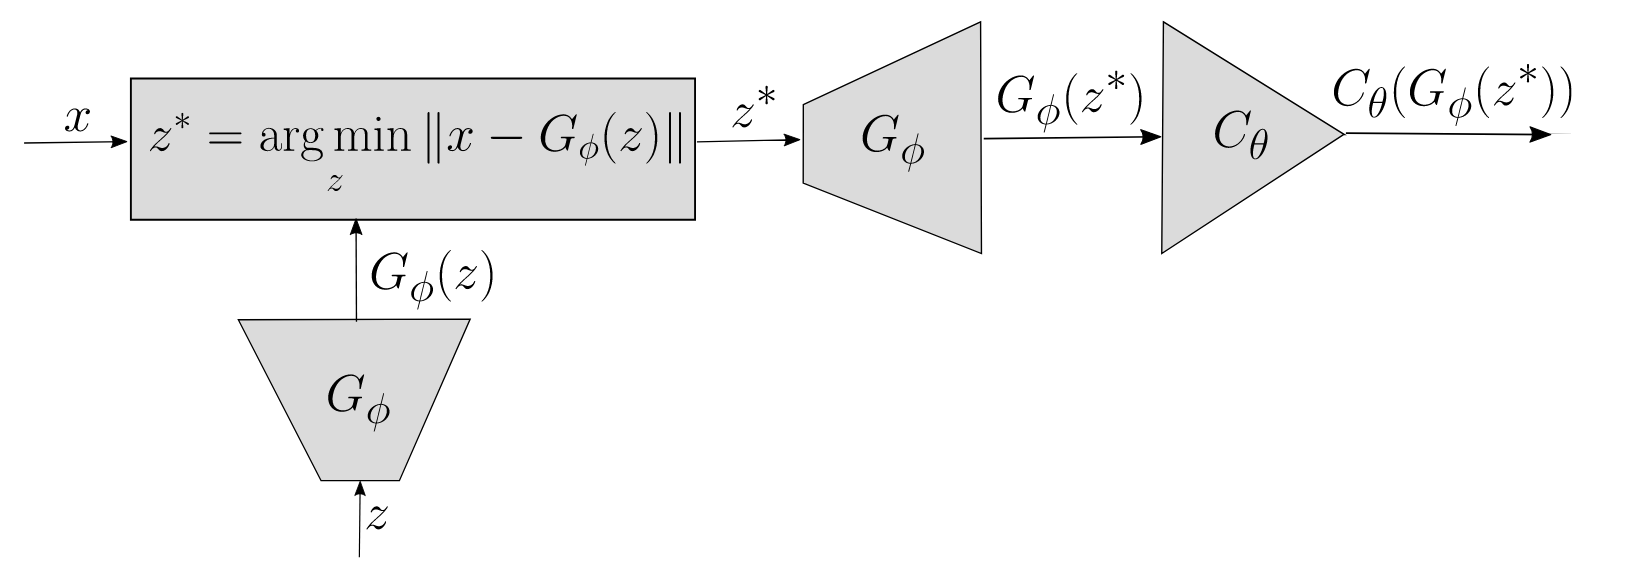
\includegraphics[scale=0.13]{./INC_diagram.png}
\end{figure}
    \begin{itemize}
    \item Assumes access to a well trained generative model for the manifold of natural images \cite{ilyas2017}
    \end{itemize}
    \begin{enumerate}
        \item Project the image onto the range of the generative model by minimizing:
        $z^* = argmin_z ||G(z) - x||_2$
        \item If the projection is far from the original image we conclude that it is an unnatural image and reject it
        $G(z^*) \geq \eta$
        \item Otherwise, classify the projection of the image:
        $C_\theta(G(z^*))$
    \end{enumerate}
\end{frame}

\begin{frame}[fragile]{Critique of INC Projection}
\begin{columns}
\begin{column}{0.5\textwidth}
 \begin{figure}[H]
    \caption{Swiss roll data $\in \mathbb{R}^2$}
    \centering
    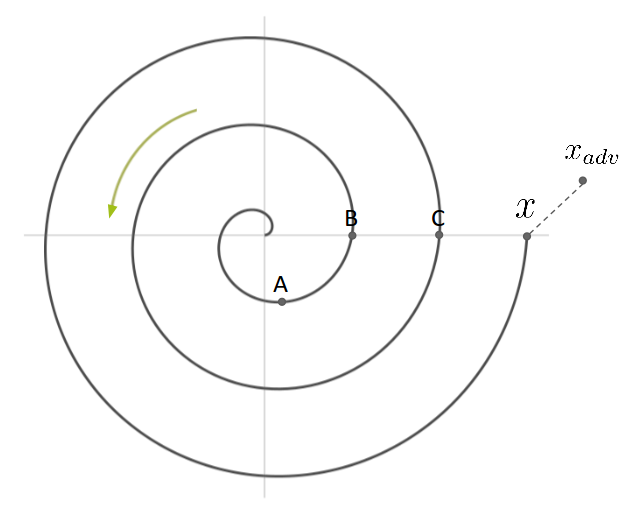
\includegraphics[scale=0.25]{./swiss.png}
\end{figure}
\end{column}

\begin{column}{0.5\textwidth}  %%<--- here
 \begin{figure}[H]
    \caption{Data loss vs $z \in \mathbb{R}$}
    \centering
    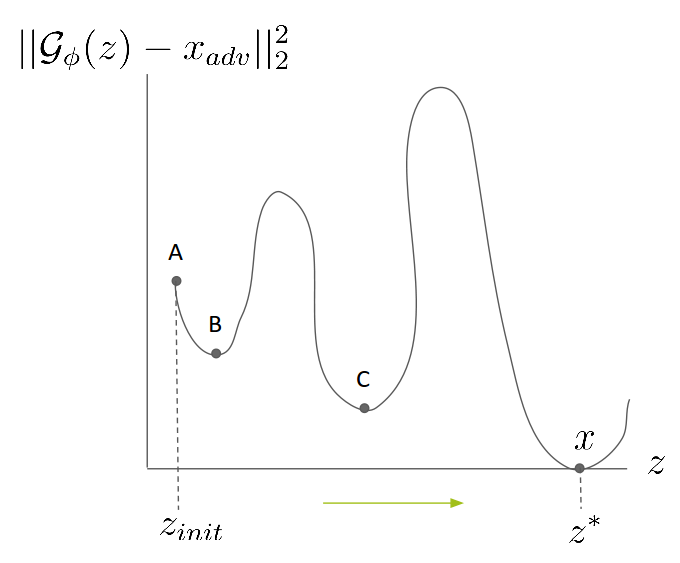
\includegraphics[scale=0.23]{./loss_swiss.png}
\end{figure}
\end{column}
\end{columns}
\begin{itemize}
    \item Minimizing the loss from a random initial point is very likely to encounter poor local minima
\end{itemize}
\end{frame}

\begin{frame}{Critique of INC Projection}

\begin{figure}[H]
    \caption{Most of the probability mass is contained in a shell of width $\frac{1}{d}$}
    \centering
    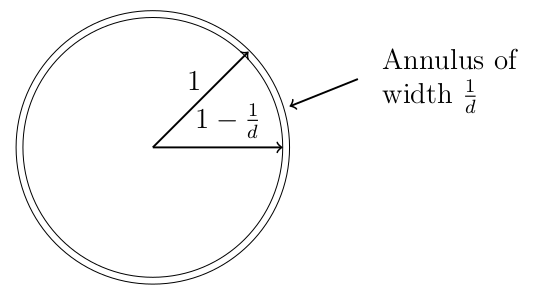
\includegraphics[scale=0.3]{./shell.png}
\end{figure}
    \begin{itemize}
        \item For Gaussian ($N(0, 1)$) random vectors in high dimensions, $||u - v||_2^2 \approx O(d)$ \cite{foundations}
        \item So a random initialization point in the latent space is far from the optimal $z^*$ w.h.p.
        \item Very likely that we will fall into a local minimum during the projection step of INC
    \end{itemize}
\end{frame}

\begin{frame}[fragile]{Fitting Encoder}
    \begin{itemize}
        \item Lets learn an Encoder which gives us a very good reference point
        \begin{itemize}
            \item Ideally, $E(X) = z^*$
            \item In practice, it is hard to match exactly: Good initial point for projection step.
        \end{itemize}
        
        \item Training Encoder that fits to GAN we use for defense.
        \begin{equation*}
            \min_{E} \mathbb{E}_{z} [||E(G(z)) - z||_2^2] + \lambda \mathbb{E}_{X} [||G(E(X)) - X||_2^2]
        \end{equation*}
        \begin{itemize}
            \item Mainly, learn in latent space first - less likely to encounter bad local optimum
            \item For regularizer, we emphasize training data since our GAN is not perfect
        \end{itemize}
    \end{itemize}
\end{frame}

\begin{frame}[fragile]{Noise Injection in Encoder Training}
    \begin{itemize}
        \item We are not only interested in inverse mapping, but also in projection
        
        \item Insert random noise in image space
        \begin{equation*}
            \min_{E} \mathbb{E}_{z, \delta} [||E(G(z) + \delta) - z||_2^2] + \lambda \mathbb{E}_{X, \delta} [||G(E(X + \delta)) - X||_2^2]
        \end{equation*}
        
        \item Two perspective on noise injection
        \begin{itemize}
            \item We teach encoder how to project points off the manifold
            \item Implicitly encouraging robustness
            \begin{align*}
                \mathbb{E}_{z, \delta} [||E(G(z) + \delta) - z||_2^2] \approx \mathbb{E}_{z, \delta} [||E(G(z)) - z + \nabla E(G(z))^T \delta||_2^2] \\
                = \mathbb{E}_{z} [||E(G(z)) - z||_2^2] + \sigma^2 \mathbb{E}_{z} [||\nabla E(G(z))||_2^2]
            \end{align*}
        \end{itemize}
    \end{itemize}
\end{frame}

\begin{frame}{Reconstruction Result on MNIST}
\begin{figure}[H]
\centering
\hspace*{-1cm}
\begin{tabular}{ccc}
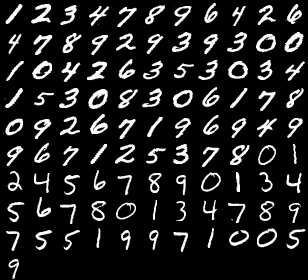
\includegraphics[width=1.5in]{reconstr_original.png} &
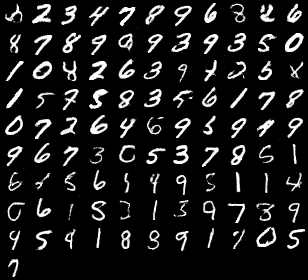
\includegraphics[width=1.5in]{reconstr_random_z.png} &
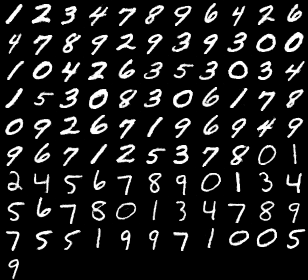
\includegraphics[width=1.5in]{reconstr_encoded.png}
\end{tabular}
\caption{Original, Reconstruction from random initial point and encoded initial point}
\end{figure}
\end{frame}

\begin{frame}{Reconstruction of Adversarial Images on F-MNIST}
\begin{figure}[H]
\centering
\hspace*{-1cm}
\begin{tabular}{ccc}
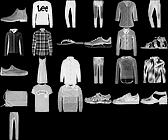
\includegraphics[width=1.5in]{f_mnist_original.png} &
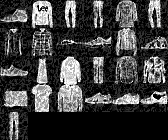
\includegraphics[width=1.5in]{f_mnist_adversarial.png} &
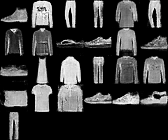
\includegraphics[width=1.5in]{f_mnist_reconstr_encoded.png} 
\end{tabular}
\caption{Noise level: eps = 0.2, PGD attack on Classifier}

Overall Accuracy \\
On Natural Image: 91.3\%, Adversarial Attack: 0\% \\
INC with random initialization: 60\% \\
INC with encoded initialization: 69.2\%
\end{figure}
\end{frame}
\appendix

\begin{frame}[allowframebreaks]{References}

  \bibliography{ref}
  \bibliographystyle{abbrv}

\end{frame}

\end{document}
